\documentclass[french, titlepage, 10pt, a4paper]{article}
\usepackage{xunicode}
\usepackage{fontspec}
\usepackage[frenchb]{babel}
\usepackage{graphicx}
\usepackage{listings}
\usepackage[T1]{fontenc}
\usepackage{kpfonts}
\usepackage[usenames,dvipsnames]{color}
\usepackage{zed}

\renewcommand{\nobreakspace}{\nobreak\ }

\author{Julien \textsc{Durillon} \and Alexandre \textsc{Garnier}}
\title{Spécification d'un gestionnaire de services}

\begin{document}

\maketitle

\section{Introduction}

Dans le cadre du module de \emph{Construction formelle du logiciel en B} du
Master ALMA de l'Université de Nantes, nous avons eu à concevoir la
spécification formelle en B d'un système des gestion de services au sein d'un
OS.\\

Il s'agit plus précisément d'une architecture basée sur un ensemble de services
accessibles par un nombre variable de processus, selon que ces services soient
en accès exclusif ou inclusif.
L'accès aux services exclusifs devra être basé sur des profils de processus, de
sorte que seuls les processus dont le profil est reconnu par un service pourront
utiliser celui-ci.

Ce faisant, on distingue trois concepts principaux au sein du projet, à savoir
les services, les processus et les profils.
Dès lors, dans notre travail de conception puis de spécification, nous avons eu
pour objectif principal de refléter cette telle répartition.\\

Dans la suite, après une analyse plus avancée du sujet, nous présenterons la
spécification formelle des différents aspects attendus du logiciel, ainsi que
les différents raffinements et implantations opérées.

Enfin, nous discuterons de la solution finale, des problèmes encontrés dans sa
conception, et des avantages et inconvénients que nous avons pu mettre à jour
quant à l'utilisation de B, et plus spécifiquement d'AtelierB.

\section{Analyse}

\subsection{Les éléments du système}

Pour pouvoir répondre aux conditions du système, nous devons manipuler les
concepts suivants:

\begin{itemize}
  \item processus: un processus identifié par un numéro;
  \item service: un service est utilisé par un processus;
  \item profile: un processus possède un profil; un service peut filtrer les
    processus autorisés via leur profil.
\end{itemize}

    \subsection{Première itération sur l'architecture}

        Dans la première version, nous avons commencé par créer une machine pour gérer
        les processus, leurs profils et les services.
        Nous nous sommes rendus compte que cette version était lourde et peu adaptée.

    \subsection{Deuxième version : modularisation}

        Les concepts \emph{processus} et \emph{profile} sont intimement liés.
        Nous allons donc séparer la conception en deux parties: d'un côté la gestion des
        processus et de leur profil, de l'autre la gestion des services.

        \subsubsection{ProcManager}

            La machine ProcManager définit le concept de \emph{processus} et celui de
            \emph{profile}. On peut ici:

                \begin{itemize}
                    \item ajouter un processus au système;
                    \item associer un processus à un profil;
                    \item enlever un processus du système.
                \end{itemize}

        \subsubsection{ServManager}
            La machine ServManager définit le concept de service, ainsi que les opérations suivantes:

            \begin{itemize}
                \item ajouter/enlever un service;
                \item associer des profils à un service;
                \item activer/désactiver un service;
                \item enregistrer un processus sur un service;
            \end{itemize}


        \subsubsection{Machine composite}


            Dans les deux machines décrites précédemment, des opérations sont
            définies qui ne fonctionnent que dans un cas chacune. Le but est de
            fournir des opérations unitaires.

            Pour gérer les différents éléments et cas, une machine Système doit être faite.
            Elle va définir les actions haut-niveau qui utiliseront les processus et les
            services.

            Dans ces actions haut-niveau, nous effectuons des tests qui nous
            permettent d'appeler une opération d'une des deux machines plus
            haut, et ainsi de relier les deux aspects.



\section{Spécification}

\subsection{Ensembles et relations: diagrammes d'Euler-Venn}

Dans la spécification formelle du projet, nous avons d'emblée veillé à ce que
les concepts de services, processus et profils soient formalisés sous forme
d'ensembles, respectivement \emph{services}, \emph{processus} et
\emph{profiles}.

\subsubsection{Gestionnaire de processus}

Dans la gestion des processus, apparaît la notion de profil d'un processus.
Tout processus est lié à un profil, cependant plusieurs processus peuvent
partager un même profil.
En outre, un profil n'a pas de raison d'exister si aucun processus ne lui est
lié.

\begin{figure}[htb]
  \centering
  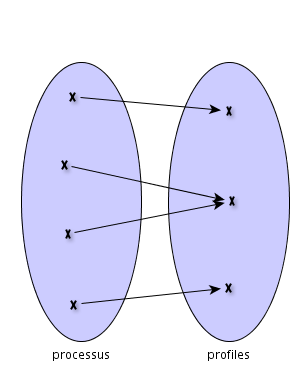
\includegraphics[width=0.4\textwidth]{proc_profile.png}
  \caption{$proc\_profile: processus \fun profiles$}
  \label{fig:proc_profile}
\end{figure}

Dès lors, nous avons formalisé une fonction totale de \emph{processus} vers
\emph{profiles}, telle que l'illustre la figure \ref{fig:proc_profile}.

\subsubsection{Gestionnaire de services}

Dans le cadre du gestionnaire de services, les relations entre ensembles
deviennent dès lors plus nombreuses, dans la mesure où sont réutilisées ici les
concepts de processus et de profils afin de mieux satisfaire à la modularité
attendue dans la gestion de services.

\begin{enumerate}

  \item Type d'un service:

    Tout service a un type d'accès, définissant si l'accès à ce service est
    contraint ou libre.
    Un service contraint devra spécifier les profils de processus pouvant
    l'utiliser.

    \begin{figure}[htb]
      \centering
      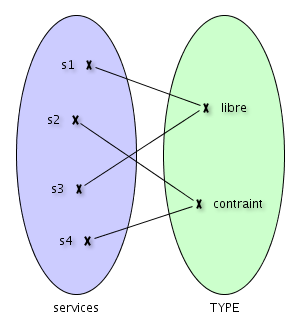
\includegraphics[width=0.4\textwidth]{type_service.png}
      \caption{$type\_service: services \fun TYPE$}
      \label{fig:type_service}
    \end{figure}

    La figure \ref{fig:type_service} montre la fonction liant un service à son
    type.

  \item Accès d'un service:

    L'accès à un service permet de spécifier si plusieurs processus peuvent
    faire appel à ce service en même temps (accès inclusif) ou non (accès
    exclusif).

    \begin{figure}[htb]
      \centering
      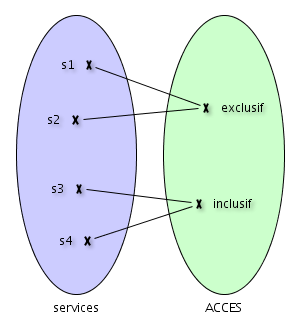
\includegraphics[width=0.4\textwidth]{acces_service.png}
      \caption{$acces\_service: services \fun ACCES$}
      \label{fig:acces_service}
    \end{figure}

    La figure \ref{fig:acces_service} montre la fonction liant un service à son
    accès.

  \item État d'un service:

    L'état d'un service permet de gérer la disponibilité ou non de celui-ci.
    Le service sera dès lors respectivement actif ou inactif.

    \begin{figure}[htb]
      \centering
      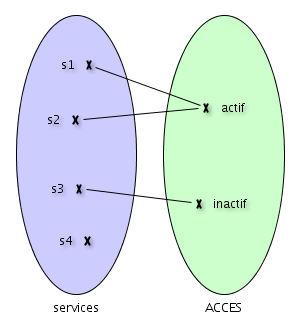
\includegraphics[width=0.4\textwidth]{etat_service.png}
      \caption{$etat\_service: services \pfun ETAT$}
      \label{fig:etat_service}
    \end{figure}

    La figure \ref{fig:etat_service} montre la fonction liant un service à son
    état.

  \item Profils que reconnaît un service contraint:

    Un service contraint est lié à un ou plusieurs profils de processus qui
    pourront dès lors l'utiliser.

    \begin{figure}[htb]
      \centering
      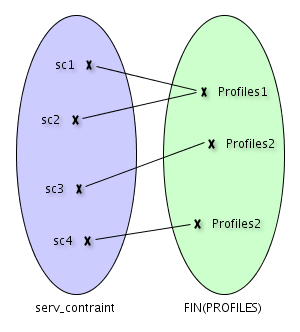
\includegraphics[width=0.4\textwidth]{serv_profiles.png}
      \caption{$serv\_profiles: serv\_contraints \fun FIN(PROFILES)$}
      \label{fig:serv_profiles}
    \end{figure}

    La figure \ref{fig:serv_profiles} montre la fonction liant un service
    contraint à ses profils de processus.

  \item Souscription d'un processus à un service:

    Un processus doit pouvoir souscrire à un service, afin de pouvoir l'utiliser
    ensuite.
    Plusieurs processus peuvent souscrire à un même service, et un processus
    peut souscrire à plusieurs services.

    \begin{figure}[htb]
      \centering
      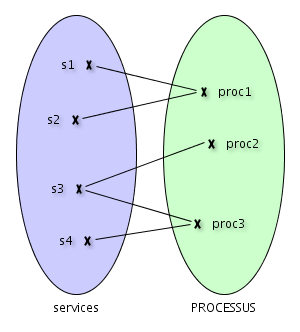
\includegraphics[width=0.4\textwidth]{serv_proc.png}
      \caption{$serv\_subscribed: services \rel PROCESSUS$}
      \label{fig:serv_subscribed}
    \end{figure}

    La figure \ref{fig:serv_subscribed} montre la relations liant des services
    à des processus leur ayant souscrit.

  \item Utilisation d'un service par un processus:

    Un processus doit dès lors être en mesure d'utiliser un service auquel il a
    souscrit.
    Pour peu que l'accès à un service soit inclusif, plusieurs processus peuvent
    l'utiliser en même temps, et un processus peut utiliser plusieurs services à
    la fois.\\

    La relation $serv\_binded: services \rel PROCESSUS$ est
    dès lors similaire à la figure \ref{fig:serv_subscribed}.

\end{enumerate}

\subsection{Opérations des machines}

\section{Organisation du travail}

Plusieurs aspects nous ont poussés à travailler ensemble sur le projet: la
gestion des projets dans AtelierB ne nous permettait pas un partage simple des
fichiers de projets; la méthode B nous étant encore assez étrangère, nous avons
préféré travailler ensemble sur les spécifications et sur le développement pour
assurer une meilleure qualité.

Dans la partie processus, il doit être possible de créer et de supprimer un
processus, d'y associer un profil.

Dans la partie service, il doit être possible de déclarer un service, de
l'activer, d'y associer les profils autorisés, d'inscrire des processus à un
service.

\section{Conclusion}

Tout au long du déroulement de ce projet, la principale difficulté aura été la
maîtrise du langage de spécification B au travers du logiciel AtelierB.

En effet, si les avantages apportés par la conception d'une preuve formelle d'un
logiciel sont indéniables du point de vue de la correction et de l'efficacité de
celui-ci, la redondance de code entre les différentes machines, raffinements et
implémentations est un inconvénient non négligeable.
De plus, le fait de devoir relancer l'ensemble des preuves dès lors qu'on
modifie l'un ou l'autre des fichiers --- dont certaines qui doivent être
effectuées via le prouveur interactif --- ne joue pas dans la simplicité
d'utilisation du logiciel.

Au-delà de ça, n'ayant pas réussi à mener à bien la preuve d'une boucle \emph
{WHILE}, nous n'avons pu implémenter l'ensemble de nos machines, et ce faisant
générer le code correspondant.

\end{document}

